\documentclass[10pt,letter,notitlepage]{article}
%Mise en page
\usepackage[left=2cm, right=2cm, lines=45, top=0.8in, bottom=0.7in]{geometry}
\usepackage{fancyhdr}
\usepackage{fancybox}
\usepackage{pdfpages} 
\renewcommand{\headrulewidth}{1.5pt}
\renewcommand{\footrulewidth}{1.5pt}
\pagestyle{fancy}
\newcommand\Loadedframemethod{TikZ}
\usepackage[framemethod=\Loadedframemethod]{mdframed}
\usepackage{tikz}
\usepackage[linesnumbered,ruled,vlined]{algorithm2e}
%\usepackage{url}
\usepackage{booktabs}
\usepackage{dsfont}
\usepackage{amssymb,amsmath}
\usepackage{xspace}
\usepackage{graphicx}
\graphicspath{ {./images/} }


\usepackage{stmaryrd}
\newcommand{\pred}[1]{\llbracket#1\rrbracket}


\lhead{
\textbf{University of Waterloo}
}
\rhead{\textbf{2021 Winter}
}
\chead{\textbf{
CS480/680
 }}

\newcommand{\RR}{\mathds{R}}
\newcommand{\sign}{\mathop{\mathrm{sign}}}
\newcommand{\argmin}{\mathop{\mathrm{argmin}}}
\newcommand{\zero}{\mathbf{0}}
\newcommand{\one}{\mathbf{1}}
\newcommand{\bv}{\mathbf{b}}
\newcommand{\wv}{\mathbf{w}}
\newcommand{\xv}{\mathbf{x}}
\newcommand{\yv}{\mathbf{y}}
\newcommand{\rv}{\mathbf{r}}
\newcommand{\inner}[2]{\langle #1, #2 \rangle}
\newcommand{\red}[1]{{\color{red}#1}}
\newcommand{\blue}[1]{{\color{blue}#1}}
\newcommand{\magenta}[1]{{\color{magenta}#1}}
\newcommand{\Xv}{\mathbf{X}}
\newcommand{\Yv}{\mathbf{Y}}
\newcommand{\EE}{\mathds{E}}
\newcommand{\pv}{\mathbf{p}}



\newcommand{\ea}{{et al.}\xspace}
\newcommand{\eg}{{e.g.}\xspace}
\newcommand{\ie}{{i.e.}\xspace}
\newcommand{\iid}{{i.i.d.}\xspace}
\newcommand{\cf}{{cf.}\xspace}
\newcommand{\wrt}{{w.r.t.}\xspace}
\newcommand{\aka}{{a.k.a.}\xspace}
\newcommand{\etc}{{etc.}\xspace}

\newcommand{\ans}[1]{{\color{orange}\textsf{Ans}: #1}}


\lfoot{}
\cfoot{\textbf{Gautam Kamath (gckamath@uwaterloo.ca) \textcopyright 2021}}

%================================
%================================

\setlength{\parskip}{1cm}
\setlength{\parindent}{1cm}
\tikzstyle{titregris} =
[draw=gray,fill=white, shading = exersicetitle, %
text=gray, rectangle, rounded corners, right,minimum height=.3cm]
\pgfdeclarehorizontalshading{exersicebackground}{100bp}
{color(0bp)=(green!40); color(100bp)=(black!5)}
\pgfdeclarehorizontalshading{exersicetitle}{100bp}
{color(0bp)=(red!40);color(100bp)=(black!5)}
\newcounter{exercise}
\renewcommand*\theexercise{exercice \textbf{Exercice}~n\arabic{exercise}}
\makeatletter
\def\mdf@@exercisepoints{}%new mdframed key:
\define@key{mdf}{exercisepoints}{%
\def\mdf@@exercisepoints{#1}
}

\mdfdefinestyle{exercisestyle}{%
outerlinewidth=1em,outerlinecolor=white,%
leftmargin=-1em,rightmargin=-1em,%
middlelinewidth=0.5pt,roundcorner=3pt,linecolor=black,
apptotikzsetting={\tikzset{mdfbackground/.append style ={%
shading = exersicebackground}}},
innertopmargin=0.1\baselineskip,
skipabove={\dimexpr0.1\baselineskip+0\topskip\relax},
skipbelow={-0.1em},
needspace=0.5\baselineskip,
frametitlefont=\sffamily\bfseries,
settings={\global\stepcounter{exercise}},
singleextra={%
\node[titregris,xshift=0.5cm] at (P-|O) %
{~\mdf@frametitlefont{\theexercise}~};
\ifdefempty{\mdf@@exercisepoints}%
{}%
{\node[titregris,left,xshift=-1cm] at (P)%
{~\mdf@frametitlefont{\mdf@@exercisepoints points}~};}%
},
firstextra={%
\node[titregris,xshift=1cm] at (P-|O) %
{~\mdf@frametitlefont{\theexercise}~};
\ifdefempty{\mdf@@exercisepoints}%
{}%
{\node[titregris,left,xshift=-1cm] at (P)%
{~\mdf@frametitlefont{\mdf@@exercisepoints points}~};}%
},
}
\makeatother


%%%%%%%%%

%%%%%%%%%%%%%%%
\mdfdefinestyle{theoremstyle}{%
outerlinewidth=0.01em,linecolor=black,middlelinewidth=0.5pt,%
frametitlerule=true,roundcorner=2pt,%
apptotikzsetting={\tikzset{mfframetitlebackground/.append style={%
shade,left color=white, right color=blue!20}}},
frametitlerulecolor=black,innertopmargin=1\baselineskip,%green!60,
innerbottommargin=0.5\baselineskip,
frametitlerulewidth=0.1pt,
innertopmargin=0.7\topskip,skipabove={\dimexpr0.2\baselineskip+0.1\topskip\relax},
frametitleaboveskip=1pt,
frametitlebelowskip=1pt
}
\setlength{\parskip}{0mm}
\setlength{\parindent}{10mm}
\mdtheorem[style=theoremstyle]{exercise}{\textbf{Exercise}}

%================Liste definition--numList-and alphList=============
\newcounter{alphListCounter}
\newenvironment
{alphList}
{\begin{list}
{\alph{alphListCounter})}
{\usecounter{alphListCounter}
\setlength{\rightmargin}{0cm}
\setlength{\leftmargin}{0.5cm}
\setlength{\itemsep}{0.2cm}
\setlength{\partopsep}{0cm}
\setlength{\parsep}{0cm}}
}
{\end{list}}
\newcounter{numListCounter}
\newenvironment
{numList}
{\begin{list}
{\arabic{numListCounter})}
{\usecounter{numListCounter}
\setlength{\rightmargin}{0cm}
\setlength{\leftmargin}{0.5cm}
\setlength{\itemsep}{0cm}
\setlength{\partopsep}{0cm}
\setlength{\parsep}{0cm}}
}
{\end{list}}

\usepackage[breaklinks=true,letterpaper=true,linkcolor=magenta,urlcolor=magenta,citecolor=black]{hyperref}

\usepackage{cleveref}


%===========================================================
\begin{document}

\begin{center}
  \large{\textbf{CS480/680: Introduction to Machine Learning} \\ Homework 3\\ \red{Due: 11:59 pm, March 9, 2021}, \red{submit on Crowdmark (yet to be set up, stay tuned)}.} \\

Include your name and student number!

\end{center}

\begin{center}
Submit your writeup in pdf and all source code in a zip file (with proper documentation). Write a script for each programming exercise so that the TAs can easily run and verify your results. Make sure your code runs!

[Text in square brackets are hints that can be ignored.]
\end{center}

\begin{exercise}[Kernels (5 pts)]
      For the following questions you might find it useful to recall the definition of a matrix being positive semidefinite (PSD).
      A matrix $M \in \mathbb{R}^{d \times d}$ is PSD if and only if $x^T Mx \geq 0$ for all vectors $x \in \mathbb{R}^d$.
      Also, Taylor series are a thing.

  \begin{enumerate}
    \item (2 pt) For $x, y \in \mathbb{R}$, consider the kernel function $k(x, y) = \exp\left(-\alpha\left(x - y\right)^2\right)$.
      What is the corresponding feature map $\phi(\cdot)$ such that $\phi(x)^T \phi(y) = k(x, y)$?
      If you were using this kernel for an SVM model, would you prefer to solve the primal or dual representation? Why?

\ans{} 


    \item (1 pt) Consider the function $\frac{1}{1 - xy}$, where $x, y \in \red{(}-1, 1\red{)}$.
      Is this function a valid kernel?
      If so, write out the corresponding feature map $\phi(\cdot)$, if not, explain why.

\ans{} 
    \item (1 pt) Consider the function $\log (1 + xy)$, where $0 < x, y \in \mathbb{R}$.
      Is this function a valid kernel?
      If so, write out the corresponding feature map $\phi(\cdot)$, if not, explain why.

\ans{} 
    \item (1 pt) Consider the function $\cos(x + y)$, where $x, y \in \mathbb{R}$.
      Is this function a valid kernel?
      If so, write out the corresponding feature map $\phi(\cdot)$, if not, explain why.

\ans{} 
  \end{enumerate}
\end{exercise}
\begin{exercise}[Decision Trees (5 pts)]
Consider the dataset given below. $X_1$ and $X_2$ are the features and $Y$ is the class label:

\vskip1em
{\hspace{5cm}
\setlength{\tabcolsep}{12pt}
	\begin{tabular}{ccc}
		\toprule
		$X_1$   &  $X_2$    &  $Y$ \\
		\midrule
		0.5 & 2.5 & -- \\
		0.5 & 5.5 & + \\
		1.5 & 4.5 & -- \\
		2.5 & 1.5 & + \\
		2.5 & 4.5 & -- \\
		4.5 & 1.5 & -- \\
		4.5 & 4.5 & + \\
		\bottomrule
	\end{tabular}
}

\vskip1em

Recall that in decision trees, we pick an attribute $X_j$ and partition the dataset into two subsets according to a threshold $t$: $D_l = \{ i: X_{i,j} < t \}$ and $D_r = \{ i: X_{i,j} \geq t \}$. On each subset $D_s$, we count the frequency of positives $p_+^s$ and the frequency of negatives $p_-^s$, for $s \in \{l, r\}$. Then, we evaluate our split using the Gini index
\begin{align}
\mathrm{GI}(t, j) = \sum_{s \in \{l, r\}} \sum_{y\in\{+,-\}} p_y^s(1-p_y^s).
\end{align}
(Empty sum is treated as 0.)
\begin{enumerate}
	\item (1 pt) Consider attribute $X_1$, what is the best $t$?

\ans{} 
	\item (1 pt) Consider attribute $X_2$, what is the best $t$?

\ans{} 
	\item (1 pt) With the best $t$ for $X_1$ and $X_2$, which attribute will you choose, $X_1$ or $X_2$? Explain your answer.

\ans{} 
	\item (1 pt) Draw a Decision Tree (need not be the best one) that has $100\%$ accuracy on the given dataset.

\ans{} 
	\item (1 pt) Will your decision tree correctly classify the following test point: $X_1 = 0.5, X_2 = 7.5, Y = +$. Explain your answer.

\ans{} 
\end{enumerate}
\end{exercise}


\begin{exercise}[Adaboost (5 pts)]

	Recall the update rules of Adaboost:
	\begin{align}
	p^t_i &= \frac{w^t_i}{\sum_{j=1}^n w^t_j},  ~~ i=1, \ldots, n \\
	\label{eq:eps} \epsilon_t &= \epsilon_t(h_t) = \sum_{i=1}^n p^t_i \cdot \pred{h_t(\xv_i) \ne y_i} \\
	\label{eq:beta}\beta_t &= \frac12\log\frac{1-\epsilon_t}{\epsilon_t} \\
	\label{eq:w} w^{t+1}_i&= w^t_i \exp(- y_i \beta_t h_t(\xv_i) ),  ~~ i=1, \ldots, n.
	\end{align}
	Here we use $i$ and $t$ to index the training examples and iterations, respectively. $\pred{A} = 1$ if the event $A$ holds and 0 otherwise. \red{Unlike in class}, here $y_i \in \{\pm 1\}$ and \textbf{we also assume $h_t(\xv_i) \in \{\pm 1\}$}.
	In this exercise we offer additional insights about Adaboost.

	\begin{enumerate}
		\item (1 pt) Prove by induction that the updates defined above indeed are equivalent to what we learned in class:
		\begin{align}
		\tilde\beta_t &= \frac{\epsilon_t}{1-\epsilon_t} \\
		\tilde w^{t+1}_i & = \tilde w^t_i \tilde\beta_t^{1-|\tilde h_t(\xv_i) - \tilde y_i|},
		\end{align}
		where in class \red{we used $\tilde y_i = \tfrac{y_i+1}{2}, \tilde h(\xv_i) = \tfrac{h(\xv_i)+1}{2} \in \{ 0,1\}$.}

		[Hint: Show that $p_i^t$ remains the same under the two seemingly different updates.]

\ans{} 
		\item (1 pt) Recall in the logistic regression lecture we made the linear assumption on the log odds ratio:
		\begin{align}
		\log\frac{p(y=1 | \Xv = \xv)}{p(y=-1 | \Xv = \xv)} \approx \wv^\top \xv + b.
		\end{align}
		Adaboost in effect tries to approximate the log odds ratio using \emph{additive} functions:
		\begin{align}
		\log\frac{p(y=1 | \Xv = \xv)}{p(y=-1 | \Xv = \xv)} \approx \sum_{t=1}^T \beta_t h_t(\xv),
		\end{align}
		where each $h_t(\xv)$ is a weak classifier. Indeed, fixing $\Xv = \xv$, prove that the minimizer of the following exponential loss
		\begin{align}
		\label{eq:exp}
		\min_{H\in \RR} ~~ \EE[ \exp(- y H) | \Xv = \xv ]
		\end{align}
		is (proportional to) the log odds ratio. Here the expectation is wrt the conditional distribution $p(y | \Xv = \xv)$.

		[Any function can be approximated arbitrarily well by additive functions but clearly not by linear functions, thus the power of Adaboost.]

\ans{} 
		\item (1 pt) Suppose $h_t$ is a weak classifier whose error $\epsilon_t > 1/2$, i.e. worse than random guessing! In this case it makes sense to flip $h_t$ to $\bar h_t (\xv) = - h_t(\xv)$. Compute the error $\epsilon_t(\bar h_t)$ and the resulting $\bar \beta_t$. Do we get the same update for $w$ in \eqref{eq:w}? Explain.

\ans{} 
		\item (1 pt) Adaboost is a greedy algorithm where we find the weak classifiers sequentially. At iteration $t$, the classifiers $h_{s}, s < t$ are already found along with their coefficients $\beta_s$. Suppose $h_t$ is given by some oracle, to find the optimal coefficient $\beta_t$, we solve an empirical approximation of the exponential loss \eqref{eq:exp}:
		\begin{align}
		\label{eq:betaopt}
		\min_{\beta\in\RR} ~~ \frac{1}{n}\sum_{i=1}^n \exp(- y_i [H_{t-1}(\xv_i) + \beta h_t(\xv_i)]),
		\end{align}
		where needless to say, $H_{t-1}(\xv) := \sum_{s=1}^{t-1} \beta_s h_s(\xv)$.
		While it is possible to solve \eqref{eq:betaopt} directly, we gain more insights by defining a distribution over the training examples $(\xv_i, y_i), i=1, \ldots, n$:
		\begin{align}
		p_i^t = \frac{\exp(- y_i H_{t-1}(\xv_i))}{\sum_{i=1}^n \exp(- y_i H_{t-1}(\xv_i))},
		\end{align}
		so that we can rewrite \eqref{eq:betaopt} equivalently as:
		\begin{align}
		\label{eq:bopt}
		\min_{\beta \in \RR} ~~ \hat\EE_t \exp[- y \beta h_t(\xv)], ~~ (\xv, y) \sim \pv^t.
		\end{align}
		(Here the hat notation is to remind you that this is an empirical expectation specified by $\pv^t$ over our training data.) Let $\epsilon_t$ be defined as in \eqref{eq:eps}. Prove that the optimal $\beta$ in \eqref{eq:bopt} is given in \eqref{eq:beta}.

		[Hint: We remind again that both $y$ and $h_t(\xv)$ are $\{\pm 1\}$-valued. Split training examples according to $h_t(\xv_i) = y_i$ or not.]

\ans{} 
		\item (1 pt) What is the training error
		\begin{align}
		\epsilon_{t+1}(h_t) = \sum_{i=1}^n p^{t+1}_i \cdot \pred{h_t(\xv_i) \ne y_i}
		\end{align}
		of the weak classifier $h_t$ on the next round $t+1$? Justify your answer. You may assume $0 < \epsilon_t < 1$ so that all quantities are well-defined.

		[Hint: This exercise should be simple, given what you have done in Ex 2.4. Split training examples according to $h_t(\xv_i) = y_i$ or not.]

  \ans{} 
	\end{enumerate}

\end{exercise}

\begin{exercise}[Backpropagation (5 pts)]

Suppose we have a multilayer perceptron:

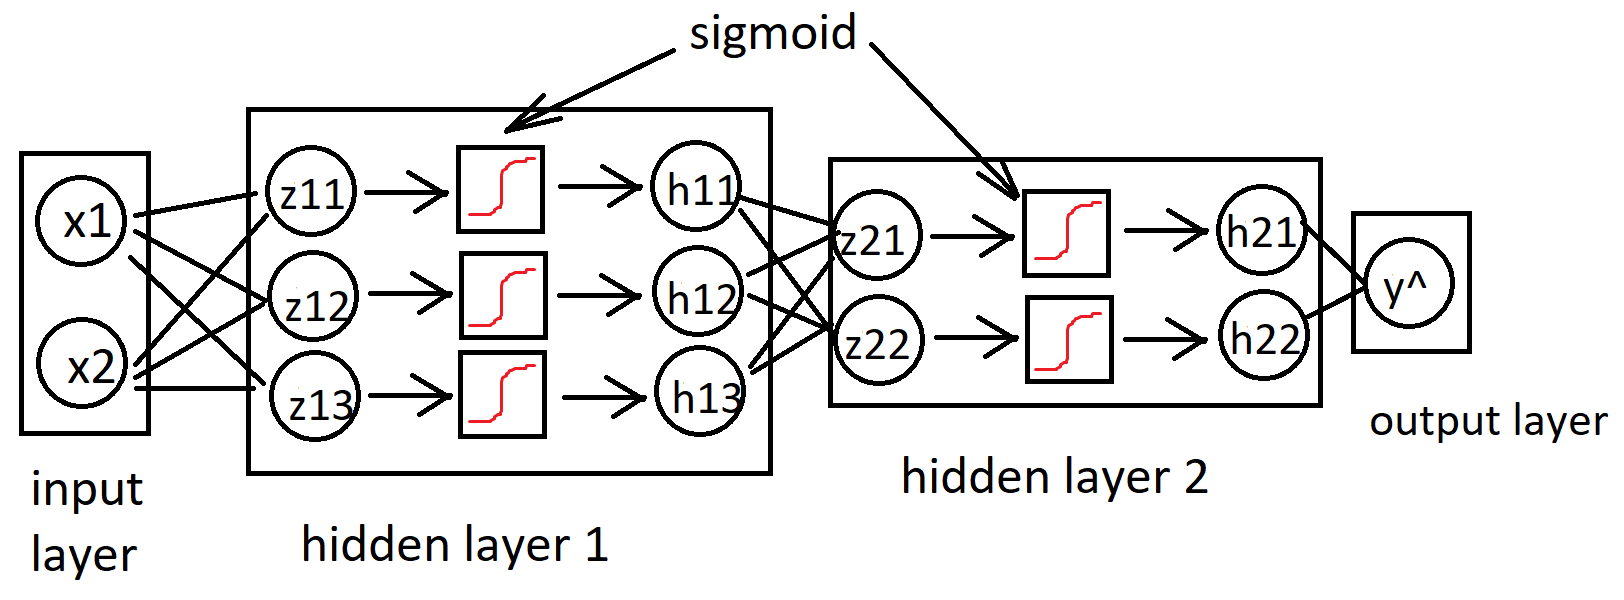
\includegraphics[scale=0.7]{1.png}
\vspace{5mm}

  Recall that the sigmoid function is $f(x) = \frac{1}{1 + e^{-x}}$.

Here
$$
z_1 = Ux + c, \quad
U = \begin{pmatrix} 1 & 0\\ 1 & 0\\ 0 & 0 \end{pmatrix}, \quad
c = \begin{pmatrix} 0\\ 1\\ 0 \end{pmatrix}, \quad
z_2 = Vh_1 + d, \quad
V = \begin{pmatrix} 1 & 0 & 0\\ 0 & 0 & 1 \end{pmatrix}, \quad
d = \begin{pmatrix} 1\\ 0 \end{pmatrix}, \quad
$$
$$
\hat{y} = \langle h_2,w \rangle + b, \quad
w = \begin{pmatrix} 0\\ 1 \end{pmatrix}, \quad
b = 0.5
$$

Also suppose that the dataset 
$$D = \{(x_1,y_1), (x_2,y_2)\} = \left\{ 
  \left(\begin{pmatrix} 1\\0\\ \end{pmatrix}, 0\right), 
\left(\begin{pmatrix} 0\\1\\ \end{pmatrix}, 1\right) \right\},$$

and loss $L$ is the mean squared error.

\begin{enumerate}
  \item (1 pt) Calculate $L$.

\ans{}
  \item (3 pt) Calculate partial derivatives of $L$ with respect to the weights of the multilayer perceptron.
    
\ans{} 
  \item (1 pt) As in gradient descent, update the weights using step size equal to 1.

\ans{} 
  \end{enumerate}

\end{exercise}

\end{document}
              
